\documentclass[10pt]{beamer}

% paquets pour le français
\usepackage[utf8]{inputenc}

\usepackage{amsmath} 
\usepackage{amsfonts}
\usepackage{amssymb}
\usepackage{mathtools}
\usepackage{xcolor} 
\usepackage{graphicx}
\usepackage{multimedia}
\usefonttheme{professionalfonts}
\usepackage{caption}
\usepackage{subcaption}\usepackage{caption}
\usepackage{hyperref}
\usepackage[absolute,overlay]{textpos}
\usetheme{Warsaw}

\DeclarePairedDelimiter\abs{\lvert}{\rvert}%

\setbeamerfont{page number in head/foot}{size=\small}
\setbeamertemplate{footline}[frame number]
\makeatletter
\newcommand\titlegraphicii[1]{\def\inserttitlegraphicii{#1}}
\titlegraphicii{}
\newcommand\titlegraphiciii[1]{\def\inserttitlegraphiciii{#1}}
\titlegraphiciii{}
\setbeamertemplate{title page}
{
  \vbox{}
   {\usebeamercolor[fg]{titlegraphic}\inserttitlegraphic\hfill\inserttitlegraphicii\hfill\inserttitlegraphiciii\par}
  \begin{centering}
    \begin{beamercolorbox}[sep=8pt,center]{institute}
      \usebeamerfont{institute}\insertinstitute
    \end{beamercolorbox}
    \begin{beamercolorbox}[sep=8pt,center]{title}
      \usebeamerfont{title}\inserttitle\par%
      \ifx\insertsubtitle\@empty%
      \else%
        \vskip0.25em%
        {\usebeamerfont{subtitle}\usebeamercolor[fg]{subtitle}\insertsubtitle\par}%
      \fi%     
    \end{beamercolorbox}%
    \vskip1em\par
    \begin{beamercolorbox}[sep=8pt,center]{date}
      \usebeamerfont{date}\insertdate
    \end{beamercolorbox}%\vskip0.5em
    \begin{beamercolorbox}[sep=8pt,center]{author}
      \usebeamerfont{author}\insertauthor
    \end{beamercolorbox}
  \end{centering}
  %\vfill
}
\makeatother
\author{Matheus Laranjeira}
\title{Asservissement référencé capteurs d'une cordée de robots sous-marins autonomes}
%\institute{Université de Toulon - Subsea Tech - Laboratoire COSMER EA 7398}
\date{Le 21 juin 2016}
\titlegraphic{\includegraphics[height=0.7cm, keepaspectratio]{Pictures/logo-utln.png}}
\titlegraphicii{\includegraphics[height=0.7cm, keepaspectratio]{Pictures/logo_subseatech.png}}
\titlegraphiciii{\includegraphics[height=0.85cm, keepaspectratio]{Pictures/COSMERlogo.png}}
\begin{document}
\begin{frame}[plain]
\maketitle
\small
{\centering\itshape Directeur de thèse : Vincent Hugel\par}
{\centering\itshape Encadrante : Claire Dune\par}
\end{frame}

\section{Le contexte de la de thèse}

\begin{frame}
\frametitle{Systèmes à ombilic}
\begin{textblock*}{12.3cm}(0.25cm, 2.5 cm) % {block width} (coords)
Typiquement utilisés par robots sous-marins télé-opérés en missions de longue durée
\end{textblock*}
\begin{textblock*}{6 cm}(0.25cm,3.5cm) % {block width} (coords)
Les avantages de la laisse :
\begin{itemize}
\item Échange de données \\
\item Autonomie energétique \\
\item Missions plus longues \\
\end{itemize}
\end{textblock*}
\begin{textblock*}{6 cm}(6.5cm,3.5cm) % {block width} (coords)
Les désavantages de la laisse :
\begin{itemize}
\item Perte de manoeuvrabilité \\
\item Exploitation difficile d'espaces confinés \\
\end{itemize}
\end{textblock*}
\begin{textblock*}{6 cm}(0.25cm,5.5cm) % {block width} (coords)
\begin{block}<2->{Cordée de robots}
\begin{itemize}
\item Couverture de zone plus étendue \\
\item Perception distribuée \\
\item Stabilisation \\
\end{itemize}
\end{block}
\end{textblock*}
\begin{textblock*}{5.2cm}(7cm,5.5cm) % {block width} (coords)
\includegraphics[scale=0.2]{Pictures/these_ifremer.png}
\end{textblock*}
\begin{textblock*}{5.2cm}(7cm,5.5cm) % {block width} (coords)
\includegraphics<2->[scale=0.2]{Pictures/cordee.png}
\end{textblock*}
\end{frame}

\begin{frame}
\begin{textblock*}{12.8cm}(0cm,1.5cm) % {block width} (coords)
\begin{center}
{\textbf{Asservissement référencé capteur d'une cordée de robots sous-marins autonomes}}  \\
\end{center}
\end{textblock*}
\begin{textblock*}{8.5cm}(0.25cm,3.5cm) % {block width} (coords)
\begin{itemize}
\item Surveillance des zones côtières, ports et chenaux
\item Eaux peu profondes – Petits robots
\item Navigation coordonnée 
\item Stabilisation de la laisse
\end{itemize}
\end{textblock*}
\begin{textblock*}{5.2cm}(6.5cm,4cm) % {block width} (coords)
\includegraphics[width=6cm, keepaspectratio]{Pictures/cordee.png}
\end{textblock*}
\end{frame}

\begin{frame}
\frametitle{Conséquences attendues sur le plan scientifique}
\begin{itemize}
\item \textbf<2->{Repérage d'amers dans l'environnement} \\
\item Fusion de données proprio- et extéroceptives \\
\item \textbf<2->{Système de navigation coordonnée} \\
\item Capacité d'auto-organisation des robots au sein de la cordée \\
\item Remplir des missions de surveillance et de reconnaissance de zones côtières en mode quasi-autonome \\
\end{itemize}
\end{frame}

\section{Première manipulation}

\begin{frame}
\frametitle{Ocean Systems Laboratory}
\begin{itemize}
\item Systèmes autonomes : planification de trajectoire, évitement d'obstacles et asservissement visuel pour robots sous-marins
\item Modélisation et analyse de capteurs : algorithmes de fusion d'information et de détection basé modèle
\end{itemize}
\begin{center}
\includegraphics<1-1>[height= 3cm]{Pictures/OSL_logo.png}
\end{center}
\begin{center}
\onslide*<1-1>{Edimbourg, Ecosse - UK}
\end{center}
\end{frame}

\begin{frame}
\frametitle{Ocean Systems Laboratory}
\begin{textblock*}{6.1cm}(0.2cm,3cm) % {block width} (coords)
\centering
\includegraphics<1->[width=6.1cm, keepaspectratio]{Pictures/OSL_piscine.jpg}
\hfill
\onslide*<1->{Piscine d'essais}
\end{textblock*}
\begin{textblock*}{6.1cm}(6.5cm,3cm) % {block width} (coords)
	\centering
	\includegraphics<2->[width=6.1cm, keepaspectratio]{Pictures/OSL_nessie.jpg}
	\hfill
	\onslide*<2->{Nessie, un robot sous-marin autonome}
\end{textblock*}
\end{frame}

\begin{frame}
\frametitle{Ocean System Laboratory}
\begin{center}
\includegraphics[height= 6cm]{Pictures/OSL_nessie_inside.jpg} \newline
5 DDL (degrés de liberté), charge utile variable
\end{center}
\end{frame}

\begin{frame}
\frametitle{Ocean System Laboratory}
\begin{textblock*}{9cm}(0.2cm,3cm) % {block width} (coords)
	\centering
	\includegraphics<1-2>[height = 5cm, keepaspectratio]{Pictures/OSL_nessie_cam.png}
\end{textblock*}
\begin{textblock*}{3.2cm}(9.4cm,3cm) % {block width} (coords)
	\centering
	\includegraphics<2-2>[ height = 5cm, angle = 0, keepaspectratio]{Pictures/OSL_nessie_DVL.png}
\end{textblock*}
\end{frame}

\begin{frame}
\begin{textblock*}{12cm}(0.4cm,1.5cm) % {block width} (coords)
\begin{block}{Objectifs}
Tester une boucle de commande en vision \\
Centrer la bouée orange dans l'image à une profondeur constante
\end{block}
\end{textblock*}
\begin{textblock*}{6.1cm}(0.4cm,3.5cm) % {block width} (coords)
\includegraphics[height=5cm, keepaspectratio]{Pictures/OSL_manip.jpg}
\end{textblock*}
\begin{textblock*}{6.1cm}(7.4cm,3.5cm) % {block width} (coords)
\includegraphics[height=5cm, keepaspectratio]{Pictures/orange_ball.png}
\end{textblock*}
\end{frame}

\begin{frame}
\frametitle{Les moyens}
\begin{block}<1->{Capteurs}
\begin{itemize}
\item Un DVL (Doppler Velocity Log) pour mesurer la vitesse du robot par rapport au fond du bassin
\item Un profondimètre
\item Un compas
\item Une camera couleur 640x480
\end{itemize}
\end{block}
\begin{block}{Commande}
\begin{itemize}
\item Une commande haut-niveau qui calcule la vitesse du robot à partir des informations visuelles
\item Une commande bas-niveau qui contrôle les propulseurs à partir de la consigne vitesse \footnotemark
\end{itemize}
\end{block}
\footnotetext[1]{C. Barbalata, V. De Carolis, M. W. Dunnigan, Y. Pétillot and D. Lane, "An adaptive controller for autonomous underwater vehicles", IROS, 2015.}
\end{frame}

\begin{frame}
\frametitle{Procedure de détection de la bouée orange}
\begin{textblock*}{12.4cm}(0.2cm, 2.5 cm) % {block width} (coords) --MAIN POINT--
Premier pas pour la mise en œuvre de l'asservissement : détection de la bouée 
\end{textblock*}
\begin{textblock*}{12cm}(0.4cm,3.5cm) % {block width} (coords)
\centering
\includegraphics[height=5cm, keepaspectratio]{Pictures/orange_ball.png}
\end{textblock*}
\end{frame}

\begin{frame}
\frametitle{Procedure de détection de la bouée orange}
\begin{itemize}
\item <1-> Détection de contours avec le filtre de Canny \footnote{J. Canny, "A Computational Approach to Edge Detection," in IEEE Transactions on Pattern Analysis and Machine Intelligence, Nov. 1986.}
\item <2-> Détection de la couleur dans l'espace HSV (teinte, saturation, brillance) \footnote{S. D. Gajbhiye and P. P. Gundewar, "A real-time color-based object tracking and occlusion handling using ARM cortex-A7" 2015 INDICON} \\
\item <3-> Opérations morphologiques pour filtrer le bruit
\end{itemize}
\end{frame}

\begin{frame}
\begin{textblock*}{12.3cm}(0.25cm, 1.5 cm) % {block width} (coords) --MAIN POINT--
\frametitle{Résultat de la détection}
\end{textblock*}
\begin{textblock*}{12.3cm}(0.25cm,2cm) % {block width} (coords)
\centering
\includegraphics[height=6.5cm, keepaspectratio]{Pictures/tracking_orange_ball.png}
\end{textblock*}
\end{frame}

\begin{frame}
\frametitle{Commande proportionnelle en translation}
\begin{textblock*}{12.3cm}(0.25cm, 2.5 cm) % {block width} (coords) --MAIN POINT--
\textbf{Objectif :} centrer la bouée dans l'image à une profondeur constante 
\end{textblock*}
\begin{textblock*} {12.3cm}(0.25cm, 3 cm)
\centering
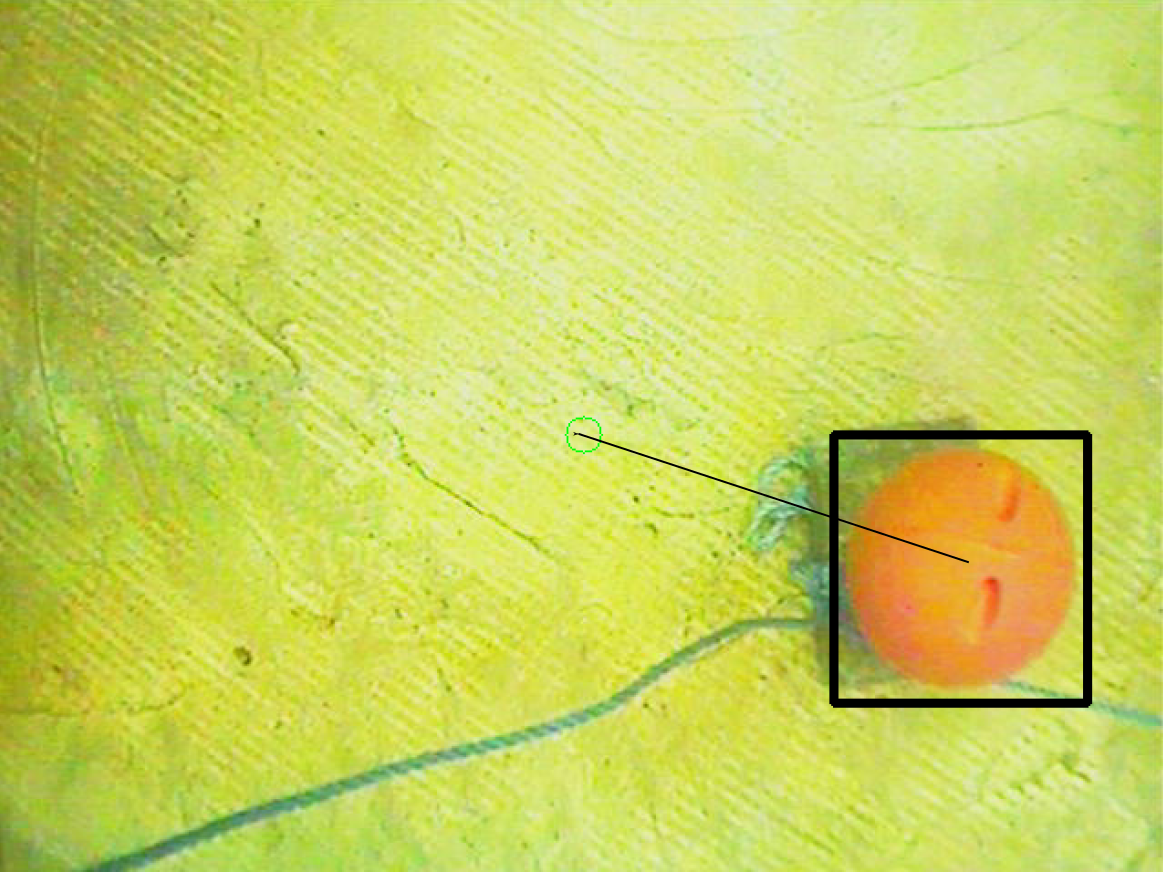
\includegraphics[height=5.5cm, keepaspectratio]{Pictures/commande_orange_ball.png}
\end{textblock*}
\end{frame}

\begin{frame}
\frametitle{Commande proportionnelle en translation}
Contrôle de 3 DDL basé sur les moments d'ordre 0 et 1 \footnote{O. Tahri and F. Chaumette, "Point-based and region-based image moments for visual servoing of planar objects" in IEEE Transactions on Robotics, Dec. 2005.} en utilisant une version simplifié de la \textbf{matrice d'interaction}
\begin{equation*}
\begin{cases}
e_x = P_x^{*} - P_x \\
e_y = P_y^{*} - P_y \\
e_z = A^{*} - A \\
\end{cases}
\end{equation*}
\begin{equation*}
\begin{bmatrix}
v_x \\ v_y \\ v_z \\ 1
\end{bmatrix}
=
\begin{bmatrix}
K_x & 0 & 0 & 0\\ 0 & K_y & 0 & 0\\ 0 & 0 & K_z & 0 \\ 0 & 0 & 0 & 1
\end{bmatrix}
\cdot
\begin{bmatrix}
e_x \\ e_y \\ e_z \\ 1
\end{bmatrix}
\end{equation*}
\begin{equation*}
\mathbf{v}_c
= \mathbf{K} \cdot
\mathbf{e}_{img}
\end{equation*}
\begin{equation*}
\mathbf{v}_r
= \mathbf{J}^{r}_c \cdot \mathbf{K} \cdot
\mathbf{e}_{img}
\end{equation*}
%\begin{equation*}
%\mathbf{v}_m
%= \mathbf{M}_{N \times4} \cdot \mathbf{J}^{r}_c \cdot \mathbf{K} \cdot
%\mathbf{e}_{img}
%\end{equation*}
% N = nombre de propulseurs
\end{frame}

\begin{frame}
\centering
\frametitle{Boucle de contrôle}
\includegraphics[width=\textwidth]{Pictures/ControlScheme.png}
\end{frame}

\begin{frame}
\frametitle{Validation en simulation}
\begin{center}
\href{run:videos/outUWSim_redbox_160422.mp4}{\includegraphics[width=0.8\textwidth, keepaspectratio]{Pictures/UWSim_nessie_redbox2.png}}
\end{center}
\end{frame}

\begin{frame}
\frametitle{Validation expérimentale}
\begin{center}
 \href{run:videos/video_OSL.mp4}{\includegraphics[width=0.8\textwidth]{Pictures/nessie2.png}}
\end{center}
\end{frame}

\section{Développement courant}

\begin{frame}
\frametitle{Gestion de la laisse à partir de la vision}
\begin{itemize}
\item Deux robots terrestres liés par une corde passive
\item Le robot de tête se déplace librement et le deuxième robot doit le suivre en analysant l'image de la corde
\end{itemize}
\end{frame}

\begin{frame}
\frametitle{La plateforme d'expérimentation}
\begin{center}
\begin{figure}
\includegraphics<1-1>[height= 6cm]{Pictures/turtle.jpg}
\caption{Le turtlebot}
\end{figure}
\end{center}
\end{frame}

\begin{frame}
\frametitle{Le scénario d'expérimentation}
\begin{center}
\begin{figure}
\includegraphics<1-1>[height= 6cm]{Pictures/turtle_set.jpg}
\end{figure}
\end{center}
\end{frame}

\begin{frame}
\frametitle{Recherche bibliographique}
\begin{itemize}
\item<1-> Les systèmes à ombilic sont utilisés depuis longtemps en robotique pour fournir de la puissance et servir de moyen de communication et de support mécanique à des robots qui opèrent en milieux sévères
\item<2-> Les robots à laisse sont utilisés en exploration planétaire afin de pouvoir accéder à des terrains irréguliers et inconnus. La laisse peut être très utile dans le processus de docking \footnote{Tsai, D.; Nesnas, I. A. D.; Zarzhitsky D. Autonomous vision-based tethered-assisted rover docking. IROS 2013} et aussi ramener le robot à la station d’atterrissage \footnote{Iqbal, J.; Heikkila, S.; Halme, A. Tether tracking and control of ROSA robotic rover. ICARCV 2008}
\item<3-> Dans l'espace, ce type de robot est utilisé en opérations de maintenance en orbite, assemblage et nettoyage de débris \footnote{Cai, J.; Huang, P.; Wang, D. Novel dynamic template matching of visual servoing for tethered space robot IEEE International Conference on Information Science and Technology, 2014}
\end{itemize}
\end{frame}

\begin{frame}
\frametitle{Tethered-assisted rover docking}
\begin{center}
\begin{figure}
\includegraphics<1-1>[height= 5cm]{Pictures/axel.png}
\includegraphics<2-2>[height= 5cm]{Pictures/RoverDocking.png}
\onslide*<1-1>{\caption{Le rover axel}}
\onslide*<2-2>{\caption{La procédure de dockage}}
\end{figure}
\end{center}
\footnotetext[5]{Tsai, D.; Nesnas, I. A. D.; Zarzhitsky D. Autonomous vision-based tethered-assisted rover docking. IROS 2013}
\end{frame}

\begin{frame}
\frametitle{Recherche bibliographique}
Récemment une méthode d'asservissement visuel a été proposée pour les robots à câbles parallèles \footnote{Dallej, T.; Gouttefarde, M.; Andreff, N.; Dahmouche, R.; Martinet, P. Vision-based modeling and control of large-dimension cable-driven parallel robots. IROS 2012.}
\begin{center}
\begin{figure}
\includegraphics<1-1>[height= 4.5cm]{Pictures/cableDriven2.png}
\includegraphics<2-2>[height= 4.5cm]{Pictures/cableDriven1.png}
\end{figure}
\end{center}
\end{frame}

\begin{frame}
\frametitle{Recherche bibliographique}
La forme de la chaînette a été prise en compte pour le transport aérien d'objets déformables afin de répartir équitablement le poids de l'objet parmi les robots \footnote{Estevez, J.; Graña, M. Robust Control Tuning by PSO of Aerial Robots Hose Transportation. Bioinspired Computation in Artificial Systems: IWINAC 2015}
\begin{center}
\begin{figure}
\includegraphics<1-1>[height= 4.5cm]{Pictures/aerialHoseTransportation.png}
\end{figure}
\end{center}
\end{frame}

\begin{frame}
\frametitle{Recherche bibliographique}
\begin{itemize}
\item<1-> Même si les systèmes à ombilic sont présents dans plusieurs domaines, la gestion de la laisse n'a pas été assez étudié dans la littérature jusqu'à présent
\item<2-> Il y a un manque d'algorithmes basés vision pour gérer la laisse et réduire les perturbations environnantes
\item<3-> Le concept de la cordée de robots peut être appliqué dans la robotique terrestre et aérienne pour le transport de matériaux déformables et l'exploration de milieux sévères
\end{itemize}
\end{frame}

%\begin{frame}
%\frametitle{Recherche bibliographique}
%Le contrôle automatique de la longueur de câble exposé a été proposé pour réduire les perturbations \footnote{Prabhakar, S.; Buckham, B. Dynamics modeling and control of a variable length remotely operated vehicle tether. OCEANS 2005}
%\begin{figure}
%\includegraphics<1-1>[height= 4.5cm]{Pictures/umbilical.png}
%\end{figure}
%\end{frame}

\begin{frame}
\frametitle{Procédure de détection de la corde orange}
\begin{itemize}
\item Détection de contours avec le filtre de Canny
\item Détection de la couleur dans l'espace HSV (teinte, saturation, brillance) \\
\item Opérations morphologiques pour filtrer le bruit
\item <2-2>Transformée de Hough pour la détection de lignes
\end{itemize}
\end{frame}

\begin{frame}
\frametitle{Résultat de la détection}
\begin{center}
\includegraphics[height=4cm, keepaspectratio]{Pictures/ropeDetection.png}
\end{center}
\end{frame}

\begin{frame}
\frametitle{Les paramètres de la chaînette}
\begin{center}
\begin{figure}
\includegraphics<1-1>[height= 6cm]{Pictures/turtle_linked.png}
\caption{Vue de dessus du scénario d'expérimentation}
\end{figure}
\end{center}
\end{frame}

\begin{frame}
\frametitle{Les paramètres de la chaînette}
\begin{center}
\begin{figure}
\includegraphics<1->[height= 5cm]{Pictures/turtle_catenary_def.png}
\end{figure}
\end{center}
\begin{equation*}
\onslide*<2-2>
{
\Sigma_C\text{ : } Y = -\frac{1}{C}\left[\cosh\left(C\left(-\frac{X}{\sin\theta}-D\right)\right)-1\right]+H+Y_{\Sigma2}
}
\onslide*<3-3>
{
\Sigma_C\text{ : } Y = -\frac{1}{\color{blue}\mathbf{C}}\left[\cosh\left({\color{blue}\mathbf{C}} \left(-\frac{X}{{\color{blue}\mathbf{\sin\theta}}}-{\color{blue}\mathbf{D}}\right)\right)-1\right]+\mathbf{\color{blue}H}+Y_{\Sigma2}
}
\end{equation*}
\end{frame}

\begin{frame}
\frametitle{Estimation des paramètres de la chaînette}
L'équation de la chaînette est composée de deux paramètres, $H$ et $\sin\theta$, puisque $C = f(H)$ et $D = g(H)$. Donc, nous pouvons affirmer que
\begin{equation*}
Y = f(X,a,b,Y_{\Sigma2})
\text{,}
\end{equation*} %
où $Y_{\Sigma2}$ est une constante et $a = \frac{H}{Hmax}$ et $b = \sin\theta$.\\
\begin{block}<2-2>{Estimation}
Après la projection de l'équation dans le plan image, nous pouvons utiliser une méthode d'optimisation, comme l'algorithme de Gauss-Newton, pour estimer les paramètres $a$ et $b$
\end{block}
\end{frame}

\begin{frame}
\frametitle{Résultat de l'estimation des paramètres}
\begin{figure}
\includegraphics<1-1>[height= 6cm]{Pictures/catenary_estim.png}
\end{figure}
\end{frame}

\begin{frame}
\frametitle{Asservissement visuel}
\begin{center}
\begin{figure}
\includegraphics<1-1>[height= 5cm]{Pictures/turtle_catenary_img_view.png}
\includegraphics<2-2>[height= 5cm]{Pictures/turtle_catenary_img_view_e1.png}
\includegraphics<3-3>[height= 5cm]{Pictures/turtle_catenary_img_view_e2.png}
\end{figure}
\end{center}
\end{frame}

\begin{frame}
\frametitle{Asservissement visuel}
Le rapport entre le mouvement du robot et l'évolution des caractéristiques visuelles est donné par une matrice d’interaction\onslide*<1-1>{\footnote{F. Chaumette and S. Hutchinson, "Visual servo control. I. Basic approaches," in IEEE Robotics and Automation Magazine, Dec. 2006}} :
\begin{equation*}
\dot{\mathbf{s}} = 
\begin{bmatrix}
	\dot{a} \\[0.3em]
	\dot{b} \\[0.3em]
\end{bmatrix}%
= \mathbf{L}\cdot %
\begin{bmatrix}
	{\mathbf{v}} \\[0.3em]
	{\mathbf{\Omega}} \\[0.3em]
\end{bmatrix}
\text{.}
\end{equation*}
À partir de la différence entre les valeurs courantes et désirées des paramètres, nous pouvons calculer la commande en vitesse :
\begin{equation*}
\mathbf{v}_c
= -\lambda\cdot\mathbf{L}^{\dagger}\cdot \mathbf{e}
\text{,}
\end{equation*}
où $\mathbf{v}_c$ est la vitesse de la caméra, $\lambda$ est un gain positif, $\mathbf{L}^{\dagger}$ est la pseudo-inverse de $\mathbf{L}$ et $\mathbf{e} = \mathbf{s} - \mathbf{s}_d$
\begin{block}<2-2>{Prochaine étape}
Valider expérimentalement le calcul de la matrice d'interaction $\mathbf{L}$ et la loi de commande
\end{block}
\end{frame}

\section{Conclusions et Perspectives}

\begin{frame}
\frametitle{Conclusions}
\begin{textblock*}{12cm}(0.5cm,3cm) % {block width} (coords)
\begin{itemize}
\item Maîtrise de l'environnement de simulation et de l'architecture de contrôle
\item Validation expérimentale d'un algorithme d'identification d'objet par sa couleur
\item Réalisation d'un asservissement visuel d'un robot sous-marin dans un environnement contrôlé
\item Validation en simulation de l'algorithme d'estimation de paramètres de la chaînette
\end{itemize}
\end{textblock*}
\end{frame}

\begin{frame}
\frametitle{Perspectives de développement}
\begin{textblock*}{12cm}(0.5cm,3cm) % {block width} (coords)
\begin{itemize}
\item Valider expérimentalement l'estimation de paramètres de la chaînette et la loi de commande en vision
\item Publier un premier article
\item Généraliser la loi de commande pour contrôler un robot sous-marin à 6 DDL
\item Validation expérimentale en mer
\item Tenir compte de l'hydrodynamique du système
\item Utiliser des câbles enroulables
\end{itemize}
\end{textblock*}
\end{frame}

\begin{frame}
\frametitle{Prochaine plateforme d'expérimentation}
\begin{figure}
\includegraphics[height= 5cm]{Pictures/blueRov.jpg}
\caption{Le BlueROV}
\end{figure}
\end{frame}

\end{document}